% ថ្នាក់ទី ១១ (វិទ្យាសាស្ត្រសង្គម) · ជំពូកទី ២ · មេរៀនទី ១ · សៀវភៅ ទំព័រ ២៧–៤៧
\chapter{អនុគមន៍អិចស្ប៉ូណង់ស្យែល}

\begin{note}[ជំពូកទី ២ ៖ អនុគមន៍អិចស្ប៉ូណង់ស្យែលនិងអនុគមន៍លោការីត]
ជំពូកនេះមានមេរៀន ៖ \textbf{១. អនុគមន៍អិចស្ប៉ូណង់ស្យែល} \quad \textbf{២. អនុគមន៍លោការីត} ។

នៅក្នុងជំពូកនេះ គេចាប់ផ្ដើមសិក្សាពីបញ្ញត្តិនៃអនុគមន៍អិចស្ប៉ូណង់ស្យែល សង់ក្រាបតាងអនុគមន៍ ដោះស្រាយសមីការ និងវិសមីការអិចស្ប៉ូណង់ស្យែល ដែលជាមធ្យោបាយសំខាន់សម្រាប់សិក្សាពីបញ្ញត្តិ ក្រាប សមីការ និងវិសមីការលោការីត ។ បន្ទាប់ពីទទួលបានបញ្ញត្តិអនុគមន៍អិចស្ប៉ូណង់ស្យែលនិងលោការីត សិស្សអាចយកចំណេះដឹងនិងបំណិនទៅដោះស្រាយចំណោទបញ្ហាដែលទាក់ទងនឹងការប្រាក់ កំណើនភ្ញៀវទេសចរដែលចូលមកទស្សនាប្រាសាទអង្គរវត្ត កំណើនប្រជាជននិងសម្រាប់ដោះស្រាយចំណោទបញ្ហាផ្សេងទៀតដែលជួបប្រទះក្នុងជីវភាពប្រចាំថ្ងៃ ។
\end{note}

\begin{objBox}[វត្ថុបំណង]
\begin{enumerate}[1]
  \item គណនាឫសទី $n$
  \item សរសេររ៉ាឌីកាល់ជាអិចស្ប៉ូណង់ស្យែល
  \item សង់ក្រាបនៃអនុគមន៍អិចស្ប៉ូណង់ស្យែល
  \item ដោះស្រាយសមីការនិងវិសមីការអិចស្ប៉ូណង់ស្យែល
  \item អនុវត្តន៍លើអនុគមន៍អិចស្ប៉ូណង់ស្យែល ។
\end{enumerate}
\end{objBox}

\section{ស្វ័យគុណ}
\subsection{និយមន័យនៃស្វ័យគុណ}

\begin{example}[ឧទាហរណ៍]
$2\times 2\times 2\times 2 = 2^4$, \quad $3\times 3\times 3\times 3\times 3 = 3^5$, \quad $(-3)(-3)(-3)(-3)(-3) = (-3)^5$ ។
\end{example}

\begin{formulaBox}[ជាទូទៅ]
\[
\underbrace{a\cdot a\cdot a\cdots a}_{n \text{ កត្តា}} = a^n
\]
កន្សោមផលគុណដែលបានមកពីការគុណនៃចំនួនដូចៗគ្នាហៅថា “ស្វ័យគុណ” ។
\end{formulaBox}

\begin{definition}[និយមន័យ]
\textbf{ស្វ័យគុណ} គឺជាកន្សោមផលគុណដែលបានមកពីការគុណនៃចំនួនដូចៗគ្នាដែលកំណត់សរសេរជាទម្រង់ $a^n$ ។
\begin{itemize}
  \item $a^n$ អានថា $a$ ស្វ័យគុណ $n$
  \item $n$ ហៅថានិទស្សន្តដែល $n$ ជាចំនួនគត់វិជ្ជមាន
  \item $a$ ហៅថាគោលនៃស្វ័យគុណ ។
\end{itemize}
\end{definition}

\begin{example}[លំហាត់គំរូ ១]
សរសេរចំនួនខាងក្រោមជាស្វ័យគុណគោល $2$ ៖ \quad ក. $16$ \quad ខ. $32$ \quad គ. $128$ ។
\ans
ក. $16 = 2\times 2\times 2\times 2 = 2^4$ \quad ខ. $32 = 2\times 2\times 2\times 2\times 2 = 2^5$ \quad គ. $128 = 2\times 2\times 2\times 2\times 2\times 2\times 2 = 2^7$ ។
\end{example}

\begin{example}[លំហាត់គំរូ ២]
សរសេរចំនួនខាងក្រោមជាស្វ័យគុណគោល $3$ ៖ \quad ក. $27$ \quad ខ. $81$ \quad គ. $243$ ។
\ans
ក. $27 = 3\times 3\times 3 = 3^3$ \quad ខ. $81 = 3\times 3\times 3\times 3 = 3^4$ \quad គ. $243 = 3\times 3\times 3\times 3\times 3 = 3^5$ ។
\end{example}

\begin{example}[លំហាត់គំរូ ៣]
ពន្លាតកន្សោមស្វ័យគុណខាងក្រោម ៖ \quad ក. $\left(\dfrac{1}{2}\right)^3$ \quad ខ. $\left(\dfrac{1}{m}\right)^3$ \quad គ. $(-10)^5$ ។
\ans
ក. $\left(\dfrac{1}{2}\right)^3 = \dfrac{1}{2}\times\dfrac{1}{2}\times\dfrac{1}{2} = \dfrac{1}{8}$ \quad ខ. $\left(\dfrac{1}{m}\right)^3 = \dfrac{1}{m}\times\dfrac{1}{m}\times\dfrac{1}{m} = \dfrac{1}{m^3}$\\
គ. $(-10)^5 = (-10)\times(-10)\times(-10)\times(-10)\times(-10) = -100\,000$ ។
\end{example}

\subsection{លក្ខណៈនៃស្វ័យគុណ}
\begin{itemize}
  \item \textbf{ផលគុណនៃស្វ័យគុណគោលដូចគ្នា ៖} គេមាន $3^2\times 3^3 = 3\times 3\times 3\times 3\times 3 = 3^5$, $3^2\times 3^3 = 3^{2+3} = 3^5$ ។ គេទាញបាន $a^m\times a^n = a^{m+n}$ ។
  \item \textbf{ស្វ័យគុណនៃស្វ័យគុណ ៖} គេមាន $(3^4)^2 = 3^4\times 3^4 = 3^{4+4} = 3^8$, $(3^4)^2 = 3^{4\times 2} = 3^8$ ។ គេទាញបាន $(a^m)^n = a^{m\times n}$ ។
  \item \textbf{ស្វ័យគុណនៃផលគុណ ៖} គេមាន $(3\times 5)^2 = (3\times 5)\times(3\times 5) = 15\times 15 = 225$ និង $3^2\times 5^2 = 9\times 25 = 225$ ។ គេទាញបាន $(ab)^n = a^n\times b^n$ ។
  \item \textbf{ស្វ័យគុណនៃផលចែក ៖} គេមាន $\left(\dfrac{3}{2}\right)^4 = \dfrac{3\times 3\times 3\times 3}{2\times 2\times 2\times 2} = \dfrac{81}{16}$, $\dfrac{3^4}{2^4} = \dfrac{81}{16}$ ។ គេទាញបាន $\left(\dfrac{a}{b}\right)^n = \dfrac{a^n}{b^n}$ $(b \ne 0)$ ។
  \item \textbf{ផលចែកនៃស្វ័យគុណគោលដូចគ្នា ៖} គេមាន $\dfrac{3^4}{3^2} = \dfrac{3\times 3\times 3\times 3}{3\times 3} = 3^2$, $\dfrac{3^4}{3^2} = 3^{4-2} = 3^2$ ។ គេទាញបាន $\dfrac{a^m}{a^n} = a^{m-n}$ $(a \ne 0)$ ។
\end{itemize}

\begin{formulaBox}[ជាទូទៅ]
បើ $a$ និង $b$ ជាចំនួនពិត ហើយ $m$ និង $n$ ជាចំនួនគត់រ៉ឺឡាទីប គេបាន ៖
\[
\begin{gathered}
a^m\times a^n = a^{m+n}, \quad (a^m)^n = a^{mn}, \quad (ab)^n = a^nb^n,\\
\left(\frac{a}{b}\right)^n = \frac{a^n}{b^n}\ (b \ne 0), \quad \frac{a^m}{a^n} = a^{m-n}\ (a \ne 0)
\end{gathered}
\]
\end{formulaBox}

\begin{example}[លំហាត់គំរូ]
សម្រួល ៖ \quad ក. $(-2)^3(-2)^7$ \quad ខ. $(3^5)^7$ \quad គ. $(4x^a\cdot y^b)(x^2\cdot y^3)$ \quad ឃ. $\left(\dfrac{x^2}{y^3}\right)^5$ \quad ង. $\dfrac{7^6}{7^5}$ \quad ច. $(5x^3y^5z^2)^4$ ។
\ans
ក. $(-2)^3(-2)^7 = (-2)^{3+7} = (-2)^{10} = 1024$ \quad ខ. $(3^5)^7 = 3^{5\times 7} = 3^{35}$ \quad គ. $(4x^a\cdot y^b)(x^2\cdot y^3) = 4x^{a+2}y^{b+3}$ \quad ឃ. $\left(\dfrac{x^2}{y^3}\right)^5 = \dfrac{(x^2)^5}{(y^3)^5} = \dfrac{x^{10}}{y^{15}}$ \quad ង. $\dfrac{7^6}{7^5} = 7^{6-5} = 7$ \quad ច. $(5x^3y^5z^2)^4 = 625x^{12}y^{20}z^8$ ។
\end{example}

\begin{pro}
សម្រួល ៖ \quad ក. $m^2\times m^8$ \quad ខ. $\dfrac{x^{11}}{x^9}$ \quad គ. $4^2 + \left(\dfrac{1}{2}\right)^4$ \quad ឃ. $\left(\dfrac{4}{9}\right)^3 \div \left(\dfrac{16}{25}\right)^2$ \quad ង. $\dfrac{(a^5b^3)^2}{a^3b^2}$ ។
\ans
ក. $m^{10}$ \quad ខ. $x^2$ \quad គ. $\dfrac{257}{16}$ \quad ឃ. $\dfrac{64}{729}\times\dfrac{625}{256} = \dfrac{625}{2916}$ \quad ង. $a^7b^4$ ។
\end{pro}

\subsection{ស្វ័យគុណចម្រាសនៃស្វ័យគុណនិងស្វ័យគុណសូន្យ}
\begin{itemize}
  \item \textbf{ស្វ័យគុណចម្រាសនៃស្វ័យគុណ ៖} $\dfrac{5^3}{5^5} = \dfrac{5\times 5\times 5}{5\times 5\times 5\times 5\times 5} = \dfrac{1}{5\times 5} = \dfrac{1}{5^2}$, $\dfrac{5^3}{5^5} = 5^{3-5} = 5^{-2}$ ។ គេសង្កេតឃើញថា $\dfrac{1}{5^2} = 5^{-2}$ ។ គេទាញបាន $\dfrac{1}{a^n} = a^{-n}$, $(a \ne 0)$ ។ គេមាន $3^{-2} = \dfrac{1}{3^2} = \dfrac{1}{9}$ និង $\dfrac{1}{3^{-2}} = \dfrac{1}{\frac{1}{3^2}} = 3^2$ ។ គេទាញបាន $a^n = \dfrac{1}{a^{-n}}$ ។
  \item \textbf{ស្វ័យគុណសូន្យ ៖} $\dfrac{5^3}{5^3} = \dfrac{5\times 5\times 5}{5\times 5\times 5} = 1$, $\dfrac{5^3}{5^3} = 5^{3-3} = 5^0$ ។ គេសង្កេតឃើញថា $\dfrac{5^3}{5^3} = 5^0 = 1$ ។ ជាទូទៅ $\dfrac{a^4}{a^4} = 1$, $\dfrac{a^4}{a^4} = a^{4-4} = a^0$ គេទាញបាន $a^0 = 1$, $(a \ne 0)$ ។
\end{itemize}
\begin{formulaBox}[ជាទូទៅ]
\[
\frac{1}{a^n} = a^{-n}\ (a \ne 0), \qquad a^0 = 1\ (a \ne 0)
\]
\end{formulaBox}

\begin{example}[លំហាត់គំរូ]
គណនា ៖ \quad ក. $-4^0$ \quad ខ. $(-4)^0$ \quad គ. $x^5 \div x^{-1}$ \quad ឃ. $(x^{-1}y^{-3})^{-1}$ \quad ង. $(2^0 + 2^{-1}) \div 3^{-2}$ \quad ច. $\left(\dfrac{a^2}{a^{-2}}\right)^{-2}$ \quad ឆ. $4\times 2^n$ \quad ជ. $\dfrac{2^m}{8}$ ។
\ans
ក. $-4^0 = -1$ \quad ខ. $(-4)^0 = 1$ \quad គ. $x^5 \div x^{-1} = x^5\times x^1 = x^6$ \quad ឃ. $(x^{-1}y^{-3})^{-1} = \dfrac{1}{x^{-1}y^{-3}} = xy^3$\\
ង. $(2^0 + 2^{-1}) \div 3^{-2} = \left(1 + \dfrac{1}{2}\right) \div \dfrac{1}{3^2} = \dfrac{3}{2}\times 9 = \dfrac{27}{2}$ \quad ច. $\left(\dfrac{a^2}{a^{-2}}\right)^{-2} = (a^4)^{-2} = \dfrac{1}{a^8}$\\
ឆ. $4\times 2^n = 2^2\times 2^n = 2^{n+2}$ \quad ជ. $\dfrac{2^m}{8} = \dfrac{2^m}{2^3} = 2^{m-3}$ ។
\end{example}

\begin{pro}
គណនា ៖ \quad ក. $(0.05)^0$ \quad ខ. $(-7^2)^0$ \quad គ. $5\times 8^0$ \quad ឃ. $\dfrac{(8^{2-2n})(16^{3-n})}{(4^{2n})^{-1}}$ \quad ង. $2\left(\dfrac{4}{m}\right)^{-2}$ \quad ច. $\left(\dfrac{6}{12m^{-3}}\right)^{-1}$ \quad ឆ. $\dfrac{2^0 + 2^{-1}}{3^{-2}}$ \quad ជ. $\dfrac{x^{-3}y^4}{x^4y^{-3}}$ \quad ឈ. $\dfrac{m^{-1} + n^{-1}}{m^{-1} - n^{-1}}$ ។
\ans
ក. $1$ \quad ខ. $1$ \quad គ. $5$ \quad ឃ. $2^{18-6n}$ \quad ង. $\dfrac{m^2}{8}$ \quad ច. $\dfrac{2}{m^3}$ \quad ឆ. $\dfrac{27}{2}$ \quad ជ. $\dfrac{y^7}{x^7}$ \quad ឈ. $\dfrac{n + m}{n - m}$ ។
\end{pro}

\section{ឫសទី \texorpdfstring{$n$}{n}}
\subsection{និយមន័យនៃឫសទី \texorpdfstring{$n$}{n}}

\begin{example}[ឧទាហរណ៍]
$16 = 2\times 2\times 2\times 2 = 2^4$, $2$ ហៅថាឫសទី $4$ នៃ $16$ ។ $16 = 4\times 4 = 4^2$, $4$ ហៅថាឫសទី $2$ នៃ $16$ ។ $16 = (-4)\times(-4) = (-4)^2$, $(-4)$ ហៅថាឫសទី $2$ នៃ $16$ ។ $27 = 3\times 3\times 3 = 3^3$, $3$ ហៅថាឫសទី $3$ នៃ $27$ ។ $-27 = (-3)\times(-3)\times(-3) = (-3)^3$, $-3$ ហៅថាឫសទី $3$ នៃ $-27$ ។
\end{example}

\begin{formulaBox}[ជាទូទៅ]
\[
a^n = \underbrace{a\times a\times\cdots\times a}_{n \text{ កត្តា}}, \quad a \text{ ហៅថាឫសទី } n \text{ នៃ } a^n
\]
\end{formulaBox}
\begin{definition}[និយមន័យ]
\textbf{ឫសទី $n$} នៃចំនួនមួយ គឺជាតម្លៃលេខណាមួយដែលគុណគ្នាដដែលៗ ចំនួន $n$ ដង ហើយស្មើនឹងចំនួនដើមនោះ ។
\end{definition}
\begin{note}[សម្គាល់]
ឫសទី $n$ នៃចំនួនមួយដែលមានសញ្ញាដូចនឹងចំនួនដើម ហៅថា “ឫសគោល” ហើយមានតែមួយគត់ ។
\end{note}

\subsection{និមិត្តសញ្ញានៃឫសទី \texorpdfstring{$n$}{n} និងការរកឫសទី \texorpdfstring{$n$}{n}}
\textbf{និមិត្តសញ្ញានៃឫសទី $n$ ៖} $\sqrt[n]{\ }$ នេះជានិមិត្តសញ្ញាពិសេសដែលមានន័យថាឫសទី $n$ ហើយត្រូវបានប្រើសម្រាប់តែឫសគោលប៉ុណ្ណោះ ។ វាជាសញ្ញារ៉ាឌីកាល់ដែល $\sqrt{\ }$ មានន័យថាឫសការេ ឬឫសទី $2$ ។ ក្នុង $\sqrt[3]{27}$ ៖ $3$ ជាសន្ទស្សន៍ $\sqrt{\ }$ ជាសញ្ញារ៉ាឌីកាល់ និង $27$ ជារ៉ាឌីកង់ ។

\textbf{ការរកឫសទី $n$ ៖}
\begin{example}[ឧទាហរណ៍ ១]
\begin{enumerate}[a]
  \item ឫសទី $3$ ឬឫសគូបនៃ $-27$ គឺ $-27 = (-3)\times(-3)\times(-3) = (-3)^3$ ។ ដូច្នេះឫសទី $3$ ឬឫសគូបនៃ $-27$ គឺ $-3$ ។
  \item ឫសទី $3$ ឬឫសគូបនៃ $27$ គឺ $27 = 3\times 3\times 3 = (3)^3$ ។ ដូច្នេះឫសទី $3$ ឬឫសគូបនៃ $27$ គឺ $3$ ។
  \item ឫសទី $5$ នៃ $-32$ គឺ $-32 = (-2)\times(-2)\times(-2)\times(-2)\times(-2) = (-2)^5$ ។ ដូច្នេះឫសទី $5$ នៃ $-32$ គឺ $-2$ ។
\end{enumerate}
\end{example}
\begin{example}[ឧទាហរណ៍ ២]
\begin{enumerate}[a]
  \item ឫសការេនៃ $16$ គឺ $16 = 4\times 4 = 4^2$ ឬ $16 = (-4)\times(-4) = (-4)^2$ ។ ដូច្នេះឫសការេនៃ $16$ មានពីរគឺ $4$ ដែលមានសញ្ញាដូចចំនួនដើមហៅថា “ឫសគោល” និង $-4$ ជាចំនួនអវិជ្ជមាន ។
  \item $\sqrt{25}$ គេបាន $\sqrt{25} = \sqrt{5^2} = 5$ ។
  \item $\sqrt[3]{-27} = \sqrt[3]{(-3)^3} = -3$ ។
  \item ឫសការេនៃ $-9$ ៖ $3^2 \ne -9$, $(-3)^2 \ne -9$ ដូច្នេះ $-9$ គ្មានឫសការេទេ ព្រោះមិនមានចំនួនពិតដូចគ្នាណាដែលគុណគ្នាពីរដងស្មើនឹង $-9$ ឡើយ ។
\end{enumerate}
\end{example}
\begin{formulaBox}[ជាទូទៅ]
ចំនួនអវិជ្ជមានគ្មានឫសការេក្នុងសំណុំចំនួនពិត ។
\end{formulaBox}

\begin{example}[លំហាត់គំរូ]
រកឫសការេនៃ ៖ \quad ក. $\dfrac{9}{25}$ \quad ខ. $\sqrt[3]{-125}$ \quad គ. $\sqrt[4]{81}$ \quad ឃ. $\sqrt{(x-1)^2}$, $\sqrt[4]{81a^4}$ \quad ង. $\sqrt{\dfrac{9}{25}}$ ។
\ans
ក. $\dfrac{9}{25} = \left(\dfrac{3}{5}\right)^2 = \left(-\dfrac{3}{5}\right)^2$ ដូច្នេះឫសការេនៃ $\dfrac{9}{25}$ មានពីរគឺ $\dfrac{3}{5}$ ជា “ឫសគោល” និង $-\dfrac{3}{5}$ ជាចំនួនអវិជ្ជមាន ។ \quad ខ. $\sqrt[3]{-125} = \sqrt[3]{(-5)^3} = -5$ \quad គ. $\sqrt[4]{81} = \sqrt[4]{3^4} = 3$ \quad ឃ. $\sqrt{(x-1)^2} = |x - 1|$ និង $\sqrt[4]{81a^4} = \sqrt[4]{3^4a^4} = 3|a|$ \quad ង. $\sqrt{\dfrac{9}{25}} = \sqrt{\left(\dfrac{3}{5}\right)^2} = \dfrac{3}{5}$ ។
\end{example}

\begin{formulaBox}[ជាទូទៅ]
$a$ ជាចំនួនពិត និង $n \ge 2$ ដែល $n$ ជាចំនួនគត់រ៉ឺឡាទីប គេបាន ៖ $\sqrt[n]{a^n} = |a|$ បើ $n$ គូ និង $\sqrt[n]{a^n} = a$ បើ $n$ សេស ។
\end{formulaBox}

\begin{example}[លំហាត់គំរូ]
គណនា ៖ \quad ក. $\sqrt[5]{-\dfrac{1}{32}}$ \quad ខ. $\sqrt{x^2 - 6x + 9}$ \quad គ. $\sqrt[6]{(-10)^6}$ \quad ឃ. $\sqrt[3]{-64x^3y^6}$ \quad ង. $\sqrt[4]{16(x-2)^4}$ \quad ច. $\sqrt[6]{(x+3)^6}$ ។
\ans
ក. $\sqrt[5]{-\dfrac{1}{32}} = \sqrt[5]{\left(-\dfrac{1}{2}\right)^5} = -\dfrac{1}{2}$ \quad ខ. $\sqrt{x^2 - 6x + 9} = \sqrt{(x-3)^2} = |x - 3|$ \quad គ. $\sqrt[6]{(-10)^6} = |-10| = 10$\\
ឃ. $\sqrt[3]{-64x^3y^6} = \sqrt[3]{(-4)^3x^3(y^2)^3} = -4xy^2$ \quad ង. $\sqrt[4]{16(x-2)^4} = 2|x - 2|$ \quad ច. $\sqrt[6]{(x+3)^6} = |x + 3|$ ។
\end{example}

\begin{pro}
គណនា ៖ \quad ក. $\sqrt{-64x^3y^6}$ \quad ខ. $\sqrt[4]{16(x-2)^4}$ \quad គ. $\sqrt[6]{(x+3)^6}$ ។
\ans
ក. គ្មានន័យក្នុង $\mathbb{R}$ (បើ $x > 0$) \quad ខ. $2|x - 2|$ \quad គ. $|x + 3|$ ។
\end{pro}

\subsection{វិធីគុណកន្សោមរ៉ាឌីកាល់}
\begin{example}[ឧទាហរណ៍]
សម្រួល $\sqrt[3]{27}\times\sqrt[3]{125}$ និង $\sqrt[3]{27\times 125}$ រួចប្រៀបធៀបចម្លើយ ។
\end{example}
គេមាន $\sqrt[3]{27}\times\sqrt[3]{125} = \sqrt[3]{3^3}\times\sqrt[3]{5^3} = 3\times 5 = 15$ និង $\sqrt[3]{27\times 125} = \sqrt[3]{3^3\times 5^3} = \sqrt[3]{(3\times 5)^3} = \sqrt[3]{15^3} = 15$ ។ គេសង្កេតឃើញថា $\sqrt[3]{27}\times\sqrt[3]{125} = \sqrt[3]{27\times 125} = 15$ ។
\begin{formulaBox}[ជាទូទៅ]
$\sqrt[n]{a}\cdot\sqrt[n]{b} = \sqrt[n]{ab}$ ចំពោះគ្រប់ចំនួនគត់ $n \ge 2$ និងគ្រប់ចំនួនវិជ្ជមាន $a$ និង $b$ ។
\end{formulaBox}
\begin{example}[លំហាត់គំរូ]
គណនា ៖ \quad ក. $\sqrt{2}\times\sqrt{8}$ \quad ខ. $\sqrt[5]{25}\times\sqrt[5]{125}$ ។
\ans
ក. $\sqrt{2}\times\sqrt{8} = \sqrt{2\times 8} = \sqrt{16} = \sqrt{4^2} = 4$ \quad ខ. $\sqrt[5]{25}\times\sqrt[5]{125} = \sqrt[5]{5^2}\times\sqrt[5]{5^3} = \sqrt[5]{5^5} = 5$ ។
\end{example}

\subsection{វិធីចែកកន្សោមរ៉ាឌីកាល់}
\begin{example}[ឧទាហរណ៍]
គណនា $\sqrt{\dfrac{64}{9}}$ និង $\dfrac{\sqrt{64}}{\sqrt{9}}$ រួចប្រៀបធៀបចម្លើយ ។
\end{example}
គេបាន $\sqrt{\dfrac{64}{9}} = \sqrt{\left(\dfrac{8}{3}\right)^2} = \dfrac{8}{3}$, $\dfrac{\sqrt{64}}{\sqrt{9}} = \dfrac{\sqrt{8^2}}{\sqrt{3^2}} = \dfrac{8}{3}$ ។ គេសង្កេតឃើញ $\sqrt{\dfrac{64}{9}} = \dfrac{\sqrt{64}}{\sqrt{9}} = \dfrac{8}{3}$ ។
\begin{formulaBox}[ជាទូទៅ]
$\dfrac{\sqrt[n]{a}}{\sqrt[n]{b}} = \sqrt[n]{\dfrac{a}{b}}$ ចំពោះគ្រប់ចំនួនគត់ $n \ge 2$ និង $a > 0$ និង $b > 0$ ។
\end{formulaBox}
\begin{example}[លំហាត់គំរូ]
គណនា ៖ \quad ក. $\dfrac{\sqrt[3]{24}}{\sqrt[3]{3}}$ \quad ខ. $\dfrac{\sqrt{125}}{\sqrt{5}}$ ។
\ans
ក. $\dfrac{\sqrt[3]{24}}{\sqrt[3]{3}} = \sqrt[3]{\dfrac{24}{3}} = \sqrt[3]{8} = 2$ \quad ខ. $\dfrac{\sqrt{125}}{\sqrt{5}} = \sqrt{\dfrac{125}{5}} = \sqrt{25} = 5$ ។
\end{example}
\begin{pro}
គណនា ៖ \quad ក. $\sqrt{\dfrac{64}{25}}$ \quad ខ. $\sqrt[3]{-\dfrac{27}{8}}$ \quad គ. $\sqrt[5]{\dfrac{32}{3125}}$ \quad ឃ. $\sqrt[4]{\dfrac{81}{2401}}$ \quad ង. $\sqrt[6]{\dfrac{1}{46656}}$ ។
\ans
ក. $\dfrac{8}{5}$ \quad ខ. $-\dfrac{3}{2}$ \quad គ. $\dfrac{2}{5}$ \quad ឃ. $\dfrac{3}{7}$ \quad ង. $\dfrac{1}{6}$ ។
\end{pro}

\subsection{ការសរសេររ៉ាឌីកាល់ជាស្វ័យគុណសនិទាន}
\begin{example}[ឧទាហរណ៍]
គណនា រួចប្រៀបធៀបចម្លើយ ។
\end{example}
\begin{enumerate}[a]
  \item $\sqrt[3]{125} = \sqrt[3]{5\times 5\times 5} = \sqrt[3]{5^3} = 5$ និង $5^{\frac{3}{3}} = 5^1 = 5$ ។ គេសង្កេតឃើញថា $\sqrt[3]{5^3} = 5^{\frac{3}{3}}$ ។
  \item $\sqrt{64} = \sqrt{8^2} = 8$ និង $8^{\frac{2}{2}} = 8^1 = 8$ ។ គេសង្កេតឃើញថា $\sqrt{8^2} = 8^{\frac{2}{2}}$ ។
  \item $\sqrt{64} = \sqrt{2^6} = \sqrt{(2^3)^2} = 2^3 = 8$ និង $2^{\frac{6}{2}} = 2^3 = 8$ ។ គេសង្កេតឃើញថា $\sqrt{2^6} = 2^{\frac{6}{2}}$ ។
\end{enumerate}
\begin{formulaBox}[ជាទូទៅ]
$\sqrt[n]{a^m} = a^{\frac{m}{n}}$ ចំពោះគ្រប់ចំនួនគត់រ៉ឺឡាទីប $n \ge 2$ និង $a > 0$ ។
\end{formulaBox}
\begin{example}[លំហាត់គំរូ]
គណនា ៖ \quad ក. $\sqrt[3]{27}$ \quad ខ. $\sqrt[5]{32^2}$ \quad គ. $\sqrt[6]{64^2}$ ។
\ans
ក. $\sqrt[3]{27} = 27^{\frac{1}{3}} = (3^3)^{\frac{1}{3}} = 3$ \quad ខ. $\sqrt[5]{32^2} = 32^{\frac{2}{5}} = (2^5)^{\frac{2}{5}} = 4$ \quad គ. $\sqrt[6]{64^2} = (2^6)^{\frac{2}{6}} = 4$ ។
\end{example}
\begin{pro}
សរសេរកន្សោមខាងក្រោមជាទម្រង់រ៉ាឌីកាល់ ៖ \quad ក. $8^{\frac{1}{3}}$ \quad ខ. $x^{\frac{1}{4}}$ \quad គ. $y^{\frac{1}{5}}$ \quad ឃ. $(a^5t^3)^{\frac{1}{2}}$ \quad ង. $(x^3y^3)^{\frac{1}{4}}$ \quad ច. $(x^3y^5)^{\frac{1}{4}}$ ។
\ans
ក. $\sqrt[3]{8} = 2$ \quad ខ. $\sqrt[4]{x}$ \quad គ. $\sqrt[5]{y}$ \quad ឃ. $\sqrt{a^5t^3}$ \quad ង. $\sqrt[4]{x^3y^3}$ \quad ច. $\sqrt[4]{x^3y^5}$ ។
\end{pro}

\subsection{វិធីគុណសន្ទស្សន៍រ៉ាឌីកាល់}
\begin{example}[ឧទាហរណ៍]
សម្រួលកន្សោម $\sqrt[3]{\sqrt[5]{x}}$ ។
\end{example}
គេមាន $\sqrt[3]{\sqrt[5]{x}} = \left(\sqrt[5]{x}\right)^{\frac{1}{3}} = x^{\frac{1}{5}\cdot\frac{1}{3}} = x^{\frac{1}{15}} = \sqrt[15]{x}$ ។ គេសង្កេតឃើញ $\sqrt[3]{\sqrt[5]{x}} = \sqrt[3\times 5]{x} = \sqrt[15]{x}$ ។
\begin{formulaBox}[ជាទូទៅ]
$\sqrt[n]{\sqrt[k]{a}} = \sqrt[nk]{a}$ ចំពោះគ្រប់ចំនួនគត់រ៉ឺឡាទីប $n \ge 2$ និង $k \ge 2$ ។
\end{formulaBox}

\subsection{ការសម្រួលសន្ទស្សន៍រ៉ាឌីកាល់}
\begin{example}[ឧទាហរណ៍]
$\sqrt[4]{25} = \sqrt[4]{5^2} = 5^{\frac{2}{4}} = 5^{\frac{1}{2}} = \sqrt{5}$, \quad $\sqrt[3]{\sqrt{27}} = \sqrt[6]{27} = (3^3)^{\frac{1}{6}} = \sqrt{3}$ ។
\end{example}
\begin{formulaBox}[ជាទូទៅ]
$\sqrt[nk]{a^{mk}} = \sqrt[n]{a^m}$ ចំពោះគ្រប់ចំនួនគត់រ៉ឺឡាទីប $n \ge 2$ និង $k \ge 2$, $a > 0$ ។\\
\textbf{លក្ខណៈឫសទី $n$ ៖} បើ $n \ge 2$, $k \ge 2$ ជាចំនួនគត់រ៉ឺឡាទីបវិជ្ជមាន $a$ និង $b$ ជាចំនួនវិជ្ជមាន គេបាន
\[
\begin{gathered}
\sqrt[n]{a}\times\sqrt[n]{b} = \sqrt[n]{ab}, \quad \sqrt[n]{\frac{a}{b}} = \frac{\sqrt[n]{a}}{\sqrt[n]{b}}\ (b \ne 0), \quad \sqrt[n]{a^m} = a^{\frac{m}{n}},\\
\sqrt[n]{\sqrt[k]{a}} = \sqrt[nk]{a}, \quad \sqrt[nk]{a^{mk}} = \sqrt[n]{a^m}
\end{gathered}
\]
\end{formulaBox}

\begin{example}[លំហាត់គំរូ]
គណនា ៖ \quad ក. $\sqrt[3]{32}$ \quad ខ. $\sqrt{2x^2 - 4x + 2}$ \quad គ. $\sqrt[3]{18a^3}\times\sqrt[3]{4b^2}$ \quad ឃ. $3\sqrt[3]{25}\times 2\sqrt[3]{5}$ \quad ង. $\sqrt[3]{\dfrac{27}{125}}$ \quad ច. $\sqrt{\dfrac{25}{x^2}}$ \quad ឆ. $\dfrac{\sqrt{16a^3}}{\sqrt{b^4}}$ \quad ជ. $\dfrac{\sqrt[3]{27x^5}}{\sqrt[3]{343y^3}}$ ។
\ans
ក. $\sqrt[3]{32} = \sqrt[3]{8\times 4} = \sqrt[3]{2^3}\times\sqrt[3]{4} = 2\sqrt[3]{4}$ \quad ខ. $\sqrt{2x^2 - 4x + 2} = \sqrt{2(x-1)^2} = |x - 1|\sqrt{2}$\\
គ. $\sqrt[3]{18a^3}\times\sqrt[3]{4b^2} = \sqrt[3]{3^2\times 2\times a^3\times 2^2\times b^2} = \sqrt[3]{2^3\times a^3\times 3^2\times b^2} = 2a\sqrt[3]{9b^2}$\\
ឃ. $3\sqrt[3]{25}\times 2\sqrt[3]{5} = 6\sqrt[3]{25\times 5} = 6\sqrt[3]{5^3} = 6\times 5 = 30$ \quad ង. $\sqrt[3]{\dfrac{27}{125}} = \dfrac{\sqrt[3]{3^3}}{\sqrt[3]{5^3}} = \dfrac{3}{5}$ \quad ច. $\sqrt{\dfrac{25}{x^2}} = \dfrac{\sqrt{25}}{\sqrt{x^2}} = \dfrac{5}{|x|}$\\
ឆ. $\dfrac{\sqrt{16a^3}}{\sqrt{b^4}} = \dfrac{\sqrt{16a^2\times a}}{\sqrt{b^4}} = \dfrac{4|a|\sqrt{a}}{b^2}$ \quad ជ. $\dfrac{\sqrt[3]{27x^5}}{\sqrt[3]{343y^3}} = \dfrac{\sqrt[3]{27x^3x^2}}{\sqrt[3]{7^3y^3}} = \dfrac{3x\sqrt[3]{x^2}}{7y}$ ។
\end{example}

\begin{pro}
គណនា ៖ \quad ក. $\sqrt[3]{0.001}\times\sqrt[3]{125}$ \quad ខ. $\sqrt[5]{x+2}\times\sqrt[5]{x-2}$ \quad គ. $\sqrt[4]{\dfrac{y}{5}}\times\sqrt[4]{\dfrac{7}{x}}$ \quad ឃ. $\sqrt[6]{512x^3y^{12}}$ \quad ង. $\dfrac{\sqrt[3]{128}}{\sqrt[3]{2}}$ \quad ច. $\dfrac{14\sqrt{128ab}}{2\sqrt{2}}$ \quad ឆ. $\dfrac{\sqrt[3]{8x^3y}}{\sqrt[3]{27y^{-2}}}$ \quad ជ. $\sqrt[3]{\dfrac{1715}{5}}$ ។
\ans
ក. $0.1\times 5 = \dfrac{1}{2}$ \quad ខ. $\sqrt[5]{x^2 - 4}$ \quad គ. $\sqrt[4]{\dfrac{7y}{5x}}$ \quad ឃ. $2y^2\sqrt{2x}$ \quad ង. $\sqrt[3]{64} = 4$ \quad ច. $7\sqrt{64ab} = 56\sqrt{ab}$ \quad ឆ. $\sqrt[3]{\dfrac{8x^3y^3}{27}} = \dfrac{2xy}{3}$ \quad ជ. $\sqrt[3]{343} = 7$ ។
\end{pro}

\section{អនុគមន៍អិចស្ប៉ូណង់ស្យែល}
\subsection{និយមន័យនៃអិចស្ប៉ូណង់ស្យែល}
\begin{example}[ឧទាហរណ៍]
គេឱ្យកន្សោមស្វ័យគុណដូចខាងក្រោម ៖ ក. $(-3)^x$ \quad ខ. $1^x$ \quad គ. $0^x$ \quad ឃ. $3^x$ ហៅថា អិចស្ប៉ូណង់ស្យែល \quad ង. $\left(\dfrac{1}{4}\right)^{-3x+2}$ ហៅថា អិចស្ប៉ូណង់ស្យែល ។
\end{example}
\begin{definition}[និយមន័យ]
\textbf{អិចស្ប៉ូណង់ស្យែល} គឺជាកន្សោមស្វ័យគុណដែលមាននិទស្សន្តជាអថេរ និងមានគោលជាចំនួនវិជ្ជមានខុសពី $1$ ។
\end{definition}

\subsection{និយមន័យនៃអនុគមន៍អិចស្ប៉ូណង់ស្យែល}
\begin{example}[ឧទាហរណ៍]
គេឱ្យទំនាក់ទំនងដូចខាងក្រោម ៖ ក. $f(x) = (-3)^x$ \quad ខ. $f(x) = 1^x$ \quad គ. $f(x) = 0^x$ \quad ឃ. $f(x) = 3^x$ ទំនាក់ទំនងនេះហៅថា អនុគមន៍អិចស្ប៉ូណង់ស្យែល \quad ង. $f(x) = 3^{-x+1}$ ទំនាក់ទំនងនេះហៅថា អនុគមន៍អិចស្ប៉ូណង់ស្យែល ។
\end{example}
\begin{definition}[និយមន័យ]
\textbf{អនុគមន៍អិចស្ប៉ូណង់ស្យែល} គឺជាអនុគមន៍ស្វ័យគុណដែលមាននិទស្សន្តជាអថេរឯករាជ្យនិងមានគោលជាចំនួនវិជ្ជមានខុសពី $1$ ។
\end{definition}

\textbf{សង្កេត ៖} រដ្ឋមួយមានប្រជាជន $1$ លាននាក់ ។ មួយទសវត្សរ៍ក្រោយមកប្រជាជនបានកើន $30\%$ ។ គំនិតខាងលើនេះ អាចឱ្យគេប៉ាន់ស្មានចំនួនប្រជាជននៃរដ្ឋនេះនៅទសវត្សរ៍ខាងមុខ តាមទំនាក់ទំនងស៊ីតធរណីមាត្រ ៖ តួទី $1$ ៖ $a_0 = 1$, ផលធៀបរួម $r = 30\% = 0.30$ ។
\begin{itemize}
  \item បើ $a_1$ ជាចំនួនប្រជាជននៃ $1$ ទសវត្សរ៍ក្រោយ ៖ $a_1 = a_0 + a_0r = a_0(1 + r) = 1(1 + 0.3) = 1.3$ ។
  \item បើ $a_2$ ជាចំនួនប្រជាជននៃ $2$ ទសវត្សរ៍ក្រោយ ៖ $a_2 = a_1 + a_1r = a_1(1 + r) = 1.3(1 + 0.3) = (1.3)^2$ ។
\end{itemize}
យើងទាញបាន $a_x = (1.3)^x$ ជាចំនួនប្រជាជនប្រែប្រួលទៅតាមអថេរ $x$ ក្នុងករណីនេះយើងបកស្រាយវាជាអនុគមន៍ $f(x) = (1.3)^x$ ។
\begin{itemize}
  \item បើ $x = 3$ នោះ $f(3) = (1.3)^3 \approx 2.19$ មានន័យថានៅ $3$ ទសវត្សរ៍ក្រោយមករដ្ឋនេះ នឹងមានប្រជាជន $2.19$ លាននាក់ ។
  \item បើ $x = -3$ នោះ $f(-3) = (1.3)^{-3} \approx 0.45$ មានន័យថានៅ $3$ ទសវត្សរ៍មុនរដ្ឋនេះមានប្រជាជនប្រមាណតែ $0.45$ លាននាក់ប៉ុណ្ណោះ ។
\end{itemize}
គេតាងក្រាបនៃអនុគមន៍ ដើម្បីឆ្លុះបញ្ចាំងកំណើននៃប្រជាជនកើនតាមឆ្នាំ ។
\begin{center}
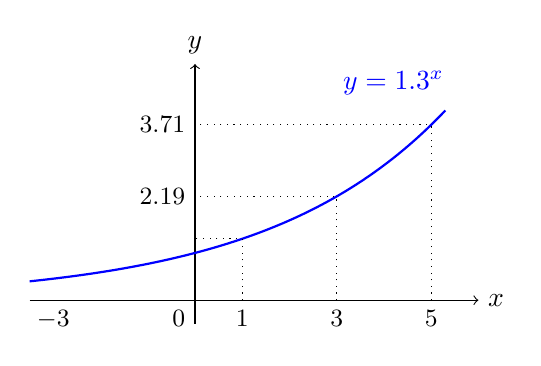
\begin{tikzpicture}[x=0.6cm,y=0.6cm]
\draw[->] (-3.5,0) -- (6,0) node[right] {$x$};
\draw[->] (0,-0.5) -- (0,5) node[above] {$y$};
\draw[thick,blue,domain=-3.5:5.3,samples=60,smooth] plot (\x,{1.3^(\x)});
\node[blue] at (4.2,4.6) {$y = 1.3^x$};
\draw[dotted] (5,0) -- (5,3.71) -- (0,3.71) node[left] {\small $3.71$};
\draw[dotted] (3,0) node[below] {\small $3$} -- (3,2.197) -- (0,2.197) node[left] {\small $2.19$};
\draw[dotted] (1,0) node[below] {\small $1$} -- (1,1.3) -- (0,1.3);
\node[below] at (5,0) {\small $5$}; \node[below] at (-3,0) {\small $-3$}; \node[below left] at (0,0) {\small $0$};
\end{tikzpicture}
\end{center}

\begin{example}[លំហាត់គំរូ ១]
សង់ក្រាបនៃអនុគមន៍ $y = 2^x$ ។
\ans
តារាងតម្លៃត្រូវគ្នានៃ $x$ និង $y$ ៖
\[
\begin{array}{|c|ccccc|}\hline
x & -2 & -1 & 0 & 1 & 2\\ \hline
y = 2^x & 0.25 & 0.50 & 1 & 2 & 4\\ \hline
\end{array}
\]
\begin{center}
\begin{tikzpicture}[x=0.7cm,y=0.7cm]
\draw[->] (-3.5,0) -- (5,0) node[right] {$x$};
\draw[->] (0,-0.5) -- (0,5.5) node[above] {$y$};
\draw[thick,blue,domain=-3.5:2.4,samples=60,smooth] plot (\x,{2^(\x)});
\node[blue] at (3,5) {$y = 2^x$};
\foreach \a in {-1,1,2} \fill (\a,{2^(\a)}) circle (1.5pt);
\fill (0,1) circle (1.5pt);
\draw[dotted] (2,0) node[below] {\small $2$} -- (2,4) -- (0,4) node[left] {\small $4$};
\draw[dotted] (1,0) node[below] {\small $1$} -- (1,2) -- (0,2) node[left] {\small $2$};
\draw[dotted] (-1,0) node[below] {\small $-1$} -- (-1,0.5) -- (0,0.5);
\node[left] at (0,1) {\small $1$};
\end{tikzpicture}
\end{center}
យើងសង្កេតឃើញថាតម្លៃ $x$ កើនគេបានតម្លៃត្រូវគ្នានៃ $y = 2^x$ កើនហើយក្រាបនៃ $y = 2^x$ កាត់អ័ក្ស $y$ ត្រង់ចំណុច $(0, 1)$ ។
\end{example}

\begin{example}[លំហាត់គំរូ ២]
សង់ក្រាបនៃអនុគមន៍ $y = \left(\dfrac{1}{2}\right)^x$ ។
\ans
តារាងតម្លៃត្រូវគ្នានៃ $x$ និង $y$ ៖
\[
\begin{array}{|c|ccccc|}\hline
x & -2 & -1 & 0 & 1 & 2\\ \hline
y = \left(\frac{1}{2}\right)^x & 4 & 2 & 1 & 0.50 & 0.25\\ \hline
\end{array}
\]
\begin{center}
\begin{tikzpicture}[x=0.7cm,y=0.7cm]
\draw[->] (-3.5,0) -- (5,0) node[right] {$x$};
\draw[->] (0,-0.5) -- (0,5.5) node[above] {$y$};
\draw[thick,blue,domain=-2.4:5,samples=60,smooth] plot (\x,{0.5^(\x)});
\node[blue] at (-3,5) {$y = \left(\frac{1}{2}\right)^x$};
\draw[dotted] (-2,0) node[below] {\small $-2$} -- (-2,4) -- (0,4) node[right] {\small $4$};
\fill (0,1) circle (1.5pt) node[right] {\small $1$};
\end{tikzpicture}
\end{center}
យើងសង្កេតឃើញតម្លៃ $x$ កើន គេបានតម្លៃត្រូវគ្នានៃ $y = \left(\dfrac{1}{2}\right)^x$ ចុះ ហើយក្រាបនៃ $y = \left(\dfrac{1}{2}\right)^x$ កាត់អ័ក្ស $oy$ ត្រង់ចំណុច $(0, 1)$ ។
\end{example}

\begin{pro}
សង់ក្រាប ៖ \quad ក. $y = 4^x$ \quad ខ. $y = \left(\dfrac{1}{4}\right)^x$ \quad គ. $y = 3^x$ \quad ឃ. $y = \left(\dfrac{1}{3}\right)^x$ ។
\ans
ក និង គ ជាក្រាបកើន ខ និង ឃ ជាក្រាបចុះ ហើយក្រាបទាំងបួនកាត់អ័ក្ស $oy$ ត្រង់ $(0, 1)$ ។ ក្រាប $y = \left(\frac{1}{4}\right)^x$ ឆ្លុះនឹងក្រាប $y = 4^x$ ធៀបនឹងអ័ក្ស $oy$ (ដូចគ្នាចំពោះ $3^x$ និង $\left(\frac{1}{3}\right)^x$) ។
\end{pro}

\section{សមីការនិងវិសមីការអិចស្ប៉ូណង់ស្យែល}
\subsection{សមីការអិចស្ប៉ូណង់ស្យែល}
\begin{example}[ឧទាហរណ៍]
គេឱ្យសមភាពដូចខាងក្រោម ៖ ក. $(-3)^x = -2187$ \quad ខ. $1^x = 1$ \quad គ. $0^x = 0$ \quad ឃ. $2^3 = 8$ \quad ង. $2^x = 8$ សមភាពដែលមានអញ្ញាតជានិទស្សន្ត និងមានគោលជាចំនួនវិជ្ជមានខុសពី $1$ ហៅថា សមីការអិចស្ប៉ូណង់ស្យែល \quad ច. $\left(\dfrac{1}{3}\right)^x = 9$ សមភាពដែលមានអញ្ញាតជានិទស្សន្ត និងមានគោលជាចំនួនវិជ្ជមានខុសពី $1$ ហៅថា សមីការអិចស្ប៉ូណង់ស្យែល ។
\end{example}
\begin{definition}[និយមន័យ]
\textbf{សមីការអិចស្ប៉ូណង់ស្យែល} ជាសមីការស្វ័យគុណដែលមាននិទស្សន្តជាអញ្ញាត និងមានគោលជាចំនួនពិតវិជ្ជមានខុសពី $1$ ។
\end{definition}

\textbf{សង្កេត ៖}
\begin{enumerate}[1]
  \item គេមានអនុគមន៍ $y = a^x$ ដែល $a$ ជាចំនួនពិតវិជ្ជមានខុសពី $1$ និងបន្ទាត់ $y = b$ ដែល $b > 0$ ។ តាមក្រាបគេសង្កេតឃើញថា បន្ទាត់ $y = b$ កាត់ក្រាបនៃអនុគមន៍ $y = a^x$ ត្រង់មួយចំណុច ។ គេបានអាប់ស៊ីសនៃចំណុចប្រសព្វជាតម្លៃ $x$ តែមួយគត់ ដែលជា\textbf{ឫស}របស់សមីការ $b = a^x$ ។ សមីការ $b = a^x$ ដែល $a$ ជាចំនួនពិតវិជ្ជមានខុសពី $1$ ហើយ $b > 0$ ហៅថា \textbf{សមីការអិចស្ប៉ូណង់ស្យែល} ។
  \item គេឱ្យអនុគមន៍អិចស្ប៉ូណង់ស្យែល $y = 2^x$ និងបន្ទាត់ $y = 8$ ។
  \item តាមក្រាបយើងសង្កេតឃើញ $2^x = 8$ មានឫសតែមួយគត់គឺ $x = 3$ មានន័យ $2^x = 2^3$ យើងទាញបាន $x = 3$ ។
\end{enumerate}
\begin{center}
\begin{tikzpicture}[x=0.55cm,y=0.55cm]
\begin{scope}
\draw[->] (-3,0) -- (3,0) node[right] {$x$}; \draw[->] (0,-0.3) -- (0,4) node[above] {$y$};
\draw[thick,blue,domain=-3:1.9,samples=50,smooth] plot (\x,{2^(\x)}); \draw[red] (-3,2) -- (3,2) node[right] {\small $y = b$};
\node[blue] at (1.5,3.8) {\small $a > 1$};
\end{scope}
\begin{scope}[xshift=4.5cm]
\draw[->] (-3,0) -- (3,0) node[right] {$x$}; \draw[->] (0,-0.3) -- (0,4) node[above] {$y$};
\draw[thick,blue,domain=-1.9:3,samples=50,smooth] plot (\x,{0.5^(\x)}); \draw[red] (-3,2) -- (3,2) node[right] {\small $y = b$};
\node[blue] at (-1.6,3.8) {\small $0 < a < 1$};
\end{scope}
\begin{scope}[xshift=9cm,y=0.4cm]
\draw[->] (-2,0) -- (4,0) node[right] {$x$}; \draw[->] (0,-0.3) -- (0,10) node[above] {$y$};
\draw[thick,green!50!black,domain=-2:3.25,samples=50,smooth] plot (\x,{2^(\x)}); \draw[red] (-1,8) -- (4,8) node[right] {\small $y = 8$};
\draw[dotted] (3,0) node[below] {\small $3$} -- (3,8);
\end{scope}
\end{tikzpicture}
\end{center}
\begin{formulaBox}[ជាទូទៅ]
ចំពោះគ្រប់ចំនួនពិត $a > 0$, $a \ne 1$ ៖ $a^x = a^y$ សមមូល $x = y$ ។
\end{formulaBox}

\begin{example}[លំហាត់គំរូ]
ដោះស្រាយសមីការ ៖ \quad ក. $4^x = 8$ \quad ខ. $3^{1-x} = \dfrac{1}{\sqrt{3}}$ \quad គ. $5\times 2^x = 40$ \quad ឃ. $18\times 3^x = 2$ \quad ង. $4^{x-1} = \left(\dfrac{1}{2}\right)^{1-3x}$ \quad ច. $5^{1-x} = (0.2)^{3x}$ ។
\ans
ក. $4^x = 8 \Leftrightarrow (2^2)^x = 2^3 \Leftrightarrow 2x = 3 \Leftrightarrow x = \dfrac{3}{2}$ ។\\
ខ. $3^{1-x} = \dfrac{1}{\sqrt{3}} = 3^{-\frac{1}{2}} \Leftrightarrow 1 - x = -\dfrac{1}{2} \Leftrightarrow x = \dfrac{3}{2}$ ។\\
គ. $5\times 2^x = 40 \Leftrightarrow 2^x = 8 = 2^3 \Leftrightarrow x = 3$ ។\\
ឃ. $18\times 3^x = 2 \Leftrightarrow 3^x = \dfrac{1}{9} = 3^{-2} \Leftrightarrow x = -2$ ។\\
ង. $4^{x-1} = \left(\dfrac{1}{2}\right)^{1-3x} \Leftrightarrow 2^{2x-2} = (2^{-1})^{1-3x} \Leftrightarrow 2x - 2 = 3x - 1 \Leftrightarrow x = -1$ ។\\
ច. $5^{1-x} = (0.2)^{3x} \Leftrightarrow 5^{1-x} = (5^{-1})^{3x} \Leftrightarrow 1 - x = -3x \Leftrightarrow x = -\dfrac{1}{2}$ ។
\end{example}

\begin{pro}
ដោះស្រាយសមីការ ៖ \quad ក. $4^x = \dfrac{1}{2}$ \quad ខ. $4^x = 1$ \quad គ. $2^x = 0$ \quad ឃ. $3^{x-1} = \left(\dfrac{1}{9}\right)^x$ \quad ង. $2^x\times 8^{1-x} = \dfrac{1}{4}$ \quad ច. $3^{x^2 - 2x} = 27$ ។
\ans
ក. $-\dfrac{1}{2}$ \quad ខ. $0$ \quad គ. គ្មានចម្លើយ \quad ឃ. $\dfrac{1}{3}$ \quad ង. $\dfrac{5}{2}$ \quad ច. $x_1 = -1$, $x_2 = 3$ ។
\end{pro}

\subsection{វិសមីការអិចស្ប៉ូណង់ស្យែល}
\begin{example}[ឧទាហរណ៍]
គេមានអនុគមន៍អិចស្ប៉ូណង់ស្យែល $y = a^x$ ដែល $a > 0$, $a \ne 1$ និង $x \in \mathbb{R}$ ។
\end{example}
\begin{itemize}
  \item បើ $a > 1$ នោះ $y = a^x$ ជាអនុគមន៍កើនជានិច្ច ចំពោះគ្រប់តម្លៃ $x$ ។ ដូច្នេះ $a^x \ge a^y$ សមមូល $x \ge y$, $a^x \le a^y$ សមមូល $x \le y$ ។
  \item បើ $0 < a < 1$ នោះ $y = a^x$ ជាអនុគមន៍ចុះជានិច្ច ចំពោះគ្រប់តម្លៃ $x$ ។ ដូច្នេះ $a^x \ge a^y$ សមមូល $x \le y$, $a^x \le a^y$ សមមូល $x \ge y$ ។
\end{itemize}

\begin{example}[លំហាត់គំរូ]
ដោះស្រាយវិសមីការ ៖ \quad ក. $2^x \le \dfrac{1}{16}$ \quad ខ. $16^n < 8^{n+1}$ \quad គ. $32^{5x+2} \ge 16^{5x}$ \quad ឃ. $(0.7)^x > 0.49$ \quad ង. $4^x - 6\times 2^x + 8 < 0$ \quad ច. $4^{3x-1} > \dfrac{1}{256}$ ។
\ans
\begin{enumerate}[a]
  \item $2^x \le \dfrac{1}{16} \Leftrightarrow 2^x \le 2^{-4} \Leftrightarrow x \le -4$ (គោល $2 > 1$) ។ ដូច្នេះ វិសមីការមានសំណុំចម្លើយ $x \in (-\infty, -4]$ ។
  \item $16^n < 8^{n+1} \Leftrightarrow (2^4)^n < 2^{3(n+1)} \Leftrightarrow 4n < 3n + 3 \Leftrightarrow n < 3$ ។ ដូច្នេះ វិសមីការមានសំណុំចម្លើយ $(-\infty, 3)$ ។
  \item $32^{5x+2} \ge 16^{5x} \Leftrightarrow 2^{5(5x+2)} \ge 2^{4(5x)} \Leftrightarrow 25x + 10 \ge 20x \Leftrightarrow x \ge -2$ ។ ដូច្នេះ វិសមីការមានសំណុំចម្លើយ $x \in [-2, +\infty)$ ។
  \item $(0.7)^x > 0.49 \Leftrightarrow (0.7)^x > (0.7)^2 \Leftrightarrow x < 2$ (គោលនៃស្វ័យគុណ $0.7 < 1$ ត្រូវប្ដូរទិសដៅវិសមីការ) ។ ដូច្នេះ $x \in (-\infty, 2)$ ។
  \item $4^x - 6\times 2^x + 8 < 0 \Leftrightarrow 2^{2x} - 6\times 2^x + 8 < 0$ ។ តាង $t = 2^x$, $t > 0$ ៖ $f(t) = t^2 - 6t + 8$ មានឫស $t = 2$, $t = 4$ ។ $f(t) < 0$ នោះ $2 < t < 4$ គឺ $2 < 2^x < 2^2$ ឬ $1 < x < 2$ ។ ដូច្នេះ $x \in (1, 2)$ ។
  \item $4^{3x-1} > \dfrac{1}{256} = 4^{-4} \Leftrightarrow 3x - 1 > -4 \Leftrightarrow x > -1$ ។ ដូច្នេះ $x \in (-1, +\infty)$ ។
\end{enumerate}
\end{example}

\begin{pro}
ដោះស្រាយវិសមីការ ៖ \quad ក. $3^x < \dfrac{1}{27}$ \quad ខ. $4^x \ge 64$ \quad គ. $16^{-x} < \dfrac{1}{256}$ \quad ឃ. $3^{x-1} < \dfrac{1}{9}$ \quad ង. $2^x\times 8^{1-x} \ge \dfrac{1}{4}$ \quad ច. $3^{x^2-2x} < 27$ ។
\ans
ក. $x < -3$ \quad ខ. $x \ge 3$ \quad គ. $x > 2$ \quad ឃ. $x < -1$ \quad ង. $x \le \dfrac{5}{2}$ \quad ច. $-1 < x < 3$ ។
\end{pro}

\section{ការអនុវត្តអនុគមន៍អិចស្ប៉ូណង់ស្យែល}
\begin{example}[ឧទាហរណ៍]
ពូសុខទិញប័ណ្ណសន្សំប្រាក់ពីធនាគារតម្លៃ $50\,000$ រៀល ដោយទទួលបានអត្រាការប្រាក់ $6\%$ ក្នុងមួយឆ្នាំ ។ បើគាត់បន្តទុកប្រាក់នោះនៅធនាគារបាន $3$ ឆ្នាំ តើប្រាក់របស់គាត់សរុបត្រូវជាប៉ុន្មាន?
\end{example}
\[
\begin{array}{lll}
\text{ឆ្នាំទី } 1 : & \text{ការប្រាក់} & 50\,000\times\frac{6}{100} = 3\,000 \text{ រៀល}\\
 & \text{ប្រាក់សរុប} & 50\,000 + 3\,000 = 53\,000 \text{ រៀល}\\
\text{ឆ្នាំទី } 2 : & \text{ការប្រាក់} & 53\,000\times\frac{6}{100} = 3\,180 \text{ រៀល}\\
 & \text{ប្រាក់សរុប} & 53\,000 + 3\,180 = 56\,180 \text{ រៀល}\\
\text{ឆ្នាំទី } 3 : & \text{ការប្រាក់} & 56\,180\times\frac{6}{100} = 3\,370.8 \text{ រៀល}\\
 & \text{ប្រាក់សរុប} & 56\,180 + 3\,370.8 = 59\,550.8 \text{ រៀល}
\end{array}
\]
ដូច្នេះ បើតាង $P$ ជាចំនួនប្រាក់ដើម ហើយ $i$ ជាអត្រាការប្រាក់ប្រចាំឆ្នាំ នោះ ៖
\begin{itemize}
  \item ចំនួនការប្រាក់នៃឆ្នាំទី $1$ គឺ $iP$
  \item ចំនួនប្រាក់សរុបនៃឆ្នាំទី $1$ គឺ $P + iP = P(1 + i)$
  \item ចំនួនប្រាក់សរុបនៃឆ្នាំទី $2$ គឺ $P(1 + i) + P(1 + i)i = P(1 + i)^2$
  \item ចំនួនប្រាក់សរុបនៃឆ្នាំទី $3$ គឺ $P(1 + i)^2 + P(1 + i)^2i = P(1 + i)^3$
  \item $\dots$ ចំនួនប្រាក់សរុបនៃឆ្នាំទី $t$ គឺ $P(1 + i)^t$ ។
\end{itemize}
\begin{formulaBox}[ជាទូទៅ]
បើតាង $P$ ជាប្រាក់ដើម $i$ ជាអត្រាការប្រាក់ប្រចាំឆ្នាំ $t$ ជាចំនួនឆ្នាំ នោះចំនួនប្រាក់សរុបគឺ $A = P(1 + i)^t$ ។
\end{formulaBox}
\begin{note}[សម្គាល់]
\begin{itemize}
  \item រូបមន្ត $A = P(1 + i)^t$ ប្រើបានតែក្នុងករណីទូទាត់ការប្រាក់មួយឆ្នាំម្ដង ។
  \item ករណីទូទាត់ការប្រាក់មួយឆមាសម្ដង គេប្រើ $A = P\left(1 + \dfrac{i}{2}\right)^{2t}$ ព្រោះមួយឆ្នាំទូទាត់ការប្រាក់ពីរដង នាំឱ្យ $t$ ឆ្នាំទូទាត់ $2t$ ហើយមួយឆ្នាំទទួលការប្រាក់ $i$ នាំឱ្យមួយឆមាសទទួលអត្រាការប្រាក់ $\dfrac{i}{2}$ ។
  \item ករណីទូទាត់ការប្រាក់មួយត្រីមាសម្ដង គេប្រើ $A = P\left(1 + \dfrac{i}{4}\right)^{4t}$ ព្រោះមួយឆ្នាំទូទាត់ការប្រាក់បួនដង នាំឱ្យ $t$ ឆ្នាំទូទាត់ $4t$ ហើយមួយឆ្នាំទទួលការប្រាក់ $i$ នាំឱ្យមួយត្រីមាសទទួលការប្រាក់ $\dfrac{i}{4}$ ។
\end{itemize}
\end{note}
\begin{formulaBox}[ជាទូទៅ]
បើ $n$ ជាចំនួនដងនៃការទូទាត់ការប្រាក់ក្នុងមួយឆ្នាំ គេបានរូបមន្ត $A = P\left(1 + \dfrac{i}{n}\right)^{nt}$ ។
\end{formulaBox}

\begin{example}[លំហាត់គំរូ ១]
នៅឆ្នាំ $1987$ អ្នកវិនិយោគទុនម្នាក់បានទិញដីមួយកន្លែងថ្លៃ $84\,000$ ដុល្លារ ហើយនៅឆ្នាំ $2007$ គាត់បានលក់ដីនោះវិញដោយទទួលបានតម្លៃ $49$ លានដុល្លារ ។ តើក្នុងមួយឆ្នាំអ្នកវិនិយោគទុននោះទទួលបានអត្រាការប្រាក់ចំណេញចំនួនប៉ុន្មាន បើប្រាក់របស់គាត់កើនពី $84\,000$ ដុល្លារដល់ $49$ លានដុល្លារក្នុងរយៈពេល $20$ ឆ្នាំ ។
\ans
តាង $i$ ជាអត្រាការប្រាក់ចំណេញ ។ គេបាន $84\,000(1 + i)^{20} = 49\,000\,000$ ឬ $(1 + i)^{20} = \dfrac{49\,000}{84}$ (លើកឫសទី $20$) ៖ $1 + i \approx 1.375$ ឬ $i \approx 0.375$ ។ ដូច្នេះ ក្នុងមួយឆ្នាំអ្នកវិនិយោគទុនទទួលបានអត្រាការប្រាក់ចំណេញ $37.5\%$ ។
\end{example}

\begin{example}[លំហាត់គំរូ ២]
នៅឆ្នាំ $1996$ មានសិស្សប្រឡងជាប់សញ្ញាបត្រមធ្យមសិក្សាទុតិយភូមិចំនួន $3\,405$ នាក់ ហើយចំនួននេះមានការកើនឡើង $30\%$ ជារៀងរាល់ឆ្នាំ ។ \quad ក. សរសេរសមីការដែលបង្ហាញចំនួនសិស្សប្រឡងជាប់ចាប់ពីឆ្នាំ $1996$ ។ \quad ខ. តើនៅឆ្នាំ $2006$ មានសិស្សប៉ុន្មាននាក់បានប្រឡងជាប់សញ្ញាបត្រមធ្យមសិក្សាទុតិយភូមិ ។
\ans
ក. ប្រើរូបមន្ត $y = C(1 + r)^t$ ដែល $C = 3\,405$ ចំនួនសិស្សប្រឡងជាប់, $r = 30\% = 0.30$ អត្រាកំណើន, $t$ ចំនួនឆ្នាំគិតពីឆ្នាំ $1996$, $y$ ចំនួនសិស្សប្រឡងជាប់ ៖ $y = 3\,405(1.30)^t$ ។ \quad ខ. $t = 2006 - 1996 = 10$ ៖ $y = 3\,405(1.30)^{10} \approx 46\,941$ ។ ដូច្នេះ ចំនួនសិស្សដែលបានប្រឡងជាប់នៅឆ្នាំ $2006$ គឺប្រហែល $46\,941$ នាក់ ។
\end{example}

\begin{example}[លំហាត់គំរូ ៣]
កសិករម្នាក់ទិញត្រាក់ទ័រមួយគ្រឿងសម្រាប់ភ្ជួរស្រែ ក្នុងតម្លៃ $50\,000$ ដុល្លារ ។ ត្រាក់ទ័រនោះចុះថ្លៃ $10\%$ ជារៀងរាល់ឆ្នាំ ។ រកតម្លៃត្រាក់ទ័រក្នុងរយៈពេល $7$ ឆ្នាំក្រោយ ។
\ans
ប្រើរូបមន្ត $y = C(1 - r)^t$ ដែល $C = 50\,000$ ជាតម្លៃទិញ, $r = 10\% = 0.10$ ជាអត្រាចុះថ្លៃ, $t = 7$ ជាចំនួនឆ្នាំ ។ គេបាន $y = 50\,000(1 - 0.10)^7 \approx 23\,914.85$ ។ ដូច្នេះ ក្នុងរយៈពេល $7$ ឆ្នាំក្រោយ តម្លៃត្រាក់ទ័រនៅសល់ត្រឹមតែ $\$23\,914.85$ ។
\end{example}

\begin{pro}
\begin{enumerate}[a]
  \item ពូស៊ុយបានយកប្រាក់មួយចំនួនទៅផ្ញើនៅធនាគារមួយ ដោយទទួលបានអត្រាការប្រាក់ $9\%$ ក្នុងមួយឆ្នាំ ។ រយៈពេល $5$ ឆ្នាំក្រោយមក គាត់បានដកប្រាក់ពីធនាគារនោះវិញ ដោយទទួលបានប្រាក់សរុបចំនួន $1\,000$ ដុល្លារ ។ តើពូស៊ុយមានប្រាក់ដើមចំនួនប៉ុន្មាន?
  \item មនុស្សម្នាក់មានអាយុ $20$ ឆ្នាំ បានយកប្រាក់ $1\,000$ ដុល្លារ ទៅផ្ញើនៅធនាគារមួយ ដោយទទួលបានអត្រាការប្រាក់ $12\%$ ក្នុងមួយឆ្នាំ ។ តើគាត់មានប្រាក់សរុបចំនួនប៉ុន្មាន បើបច្ចុប្បន្នគាត់មានអាយុ $60$ ឆ្នាំ?
  \item មនុស្សម្នាក់បានទិញរថយន្តថ្មីមួយគ្រឿងម៉ាកតូយ៉ូតាកាម៉ារី ក្នុងតម្លៃ $3\,900$ ដុល្លារ ។ រថយន្តនោះចុះថ្លៃ $14\%$ ជារៀងរាល់ឆ្នាំ ។ រកតម្លៃរថយន្តក្នុងរយៈពេល $10$ ឆ្នាំក្រោយ ។
\end{enumerate}
\ans
ក. $P = \dfrac{1\,000}{(1.09)^5} \approx \$649.93$ \quad ខ. $A = 1\,000(1.12)^{40} \approx \$93\,050.97$ \quad គ. $3\,900(0.86)^{10} \approx \$863.08$ ។
\end{pro}

\section*{លំហាត់អនុវត្តន៍}
\begin{enumerate}[1]
  \item គណនាតម្លៃនៃកន្សោមខាងក្រោម ៖
  \begin{tasks}(4)
    \task $\sqrt{16}$
    \task $\sqrt{225}$
    \task $\sqrt{144}$
    \task $\sqrt[3]{0.008(y-2)^3}$
    \task $\sqrt{(-6x)^2}$
    \task $\sqrt[3]{27}$
    \task $-\sqrt[3]{64}$
    \task $\sqrt[3]{-64x^3}$
  \end{tasks}
  \ans
  ក. $4$ \quad ខ. $15$ \quad គ. $12$ \quad ឃ. $0.2(y - 2)$ \quad ង. $6|x|$ \quad ច. $3$ \quad ឆ. $-4$ \quad ជ. $-4x$ ។
  \item សរសេរកន្សោមខាងក្រោមជាទម្រង់អិចស្ប៉ូណង់ស្យែល ៖ \quad ក. $x = \sqrt[4]{10}$ \quad ខ. $\sqrt[8]{56} = k$ \quad គ. $a = \sqrt[28]{500h}$ \quad ឃ. $b = \sqrt[x]{y}$ ។
  \ans
  ក. $x = 10^{\frac{1}{4}}$ \quad ខ. $k = 56^{\frac{1}{8}}$ \quad គ. $a = (500h)^{\frac{1}{28}}$ \quad ឃ. $b = y^{\frac{1}{x}}$ ។
  \item សម្រួលកន្សោមខាងក្រោម ៖
  \begin{tasks}(4)
    \task $\sqrt[4]{625}$
    \task $\sqrt[5]{-1}$
    \task $-\sqrt[5]{-32}$
    \task $\sqrt[5]{-\frac{1}{32}}$
    \task $\sqrt[6]{x^6}$
    \task $\sqrt[4]{(7b)^4}$
    \task $\sqrt[7]{y^7}$
    \task $\sqrt[5]{(x-2)^5}$
  \end{tasks}
  \ans
  ក. $5$ \quad ខ. $-1$ \quad គ. $2$ \quad ឃ. $-\dfrac{1}{2}$ \quad ង. $|x|$ \quad ច. $7|b|$ \quad ឆ. $y$ \quad ជ. $x - 2$ ។
  \item រកដែនកំណត់នៃអនុគមន៍ខាងក្រោម ៖
  \begin{tasks}(3)
    \task $f(x) = \sqrt{x}$
    \task $f(x) = \sqrt[3]{x}$
    \task $f(x) = \sqrt{2x + 8}$
    \task $f(x) = \sqrt{4 - 3x}$
    \task $f(x) = \sqrt{-3x^2}$
    \task $f(x) = \sqrt{x^2 + 1}$
    \task $f(x) = \dfrac{\sqrt{x}}{2x^2 - 3x - 5}$
    \task $f(x) = \dfrac{\sqrt{x + 3}}{x^2 - x - 2}$
    \task $f(x) = \dfrac{\sqrt{x + 1}}{x + |x|}$
  \end{tasks}
  \ans
  ក. $[0, +\infty)$ \quad ខ. $\mathbb{R}$ \quad គ. $[-4, +\infty)$ \quad ឃ. $\left(-\infty, \dfrac{4}{3}\right]$ \quad ង. $\{0\}$ \quad ច. $\mathbb{R}$ \quad ឆ. $\left[0, \dfrac{5}{2}\right) \cup \left(\dfrac{5}{2}, +\infty\right)$ \quad ជ. $[-3, -1) \cup (-1, 2) \cup (2, +\infty)$ \quad ឈ. $(0, +\infty)$ ។
  \item គណនាកន្សោមខាងក្រោម ៖
  \begin{tasks}(3)
    \task $\sqrt[3]{3}\times\sqrt[3]{5}$
    \task $\sqrt[4]{8}\times\sqrt[4]{9}\times\sqrt[4]{72}$
    \task $\sqrt{3a}\times\sqrt{10b}$
    \task $\sqrt{x - a}\times\sqrt{x + a}$
    \task $\sqrt{\frac{6}{x}}\times\sqrt{\frac{y}{5}}$
  \end{tasks}
  \ans
  ក. $\sqrt[3]{15}$ \quad ខ. $\sqrt[4]{5184} = \sqrt{72} = 6\sqrt{2}$ \quad គ. $\sqrt{30ab}$ \quad ឃ. $\sqrt{x^2 - a^2}$ \quad ង. $\sqrt{\dfrac{6y}{5x}}$ ។
  \item សម្រួលកន្សោមខាងក្រោម ៖ \quad ក. $\dfrac{2}{3}\sqrt{45} + \dfrac{3}{2}\sqrt[3]{16} + \dfrac{1}{4}\sqrt{72}$ \quad ខ. $x\sqrt[3]{2y} - \sqrt[3]{16x^3y} + \dfrac{x}{3}\sqrt[3]{54y}$ ។
  \ans
  ក. $2\sqrt{5} + 3\sqrt[3]{2} + \dfrac{3}{2}\sqrt{2}$ \quad ខ. $x\sqrt[3]{2y} - 2x\sqrt[3]{2y} + x\sqrt[3]{2y} = 0$ ។
  \item ប្រៀបធៀបកន្សោមខាងក្រោម ៖ \quad ក. $5\sqrt[3]{2}$ និង $2\sqrt[3]{31}$ \quad ខ. $\sqrt[3]{2}$ និង $\sqrt[12]{45}$ \quad គ. $\sqrt[6]{5}$ និង $\sqrt[8]{8}$ ។
  \ans
  ក. $5\sqrt[3]{2} = \sqrt[3]{250} > \sqrt[3]{248} = 2\sqrt[3]{31}$ \quad ខ. $\sqrt[3]{2} = \sqrt[12]{16} < \sqrt[12]{45}$ \quad គ. $\sqrt[6]{5} = \sqrt[24]{625} > \sqrt[24]{512} = \sqrt[8]{8}$ ។
  \item សម្រួលកន្សោមខាងក្រោម ៖ \quad ក. $\dfrac{\sqrt[3]{c^3 + 3c^2d + 3cd^2 + d^3}}{\sqrt{c^2 - d^2}\times\sqrt{c^2 - d^2}}$ \quad ខ. $\dfrac{\sqrt{x}}{\sqrt{x} - \sqrt{x + 1}}$ \quad គ. $\dfrac{\sqrt{p}}{\sqrt{3q^2 + 4pq + p^2}}\times\dfrac{\sqrt{p + 3q}}{\sqrt{p^2 + 6pq + 8q^2}} \div \dfrac{1}{\sqrt{p^2 + 3pq + 2q^2}}$ ។
  \ans
  ក. $\dfrac{c + d}{c^2 - d^2} = \dfrac{1}{c - d}$ \quad ខ. $-\left(x + \sqrt{x^2 + x}\right)$ \quad គ. ដោយ $3q^2 + 4pq + p^2 = (p + q)(p + 3q)$, $p^2 + 6pq + 8q^2 = (p + 2q)(p + 4q)$, $p^2 + 3pq + 2q^2 = (p + q)(p + 2q)$ ៖ លទ្ធផល $= \sqrt{\dfrac{p}{p + 4q}}$ ។
  \item សរសេរកន្សោមខាងក្រោមជាទម្រង់រ៉ាឌីកាល់ ៖ \quad ក. $8^{\frac{1}{3}}$ \quad ខ. $x^{\frac{1}{4}}$ \quad គ. $y^{\frac{1}{5}}$ \quad ឃ. $(a^5t^3)^{\frac{1}{2}}$ \quad ង. $(x^3y^3)^{\frac{1}{4}}$ \quad ច. $(x^3y^5)^{\frac{1}{4}}$ ។
  \ans
  ក. $\sqrt[3]{8} = 2$ \quad ខ. $\sqrt[4]{x}$ \quad គ. $\sqrt[5]{y}$ \quad ឃ. $\sqrt{a^5t^3}$ \quad ង. $\sqrt[4]{x^3y^3}$ \quad ច. $\sqrt[4]{x^3y^5}$ ។
  \item ដោះស្រាយសមីការខាងក្រោម ៖
  \begin{tasks}(2)
    \task $2^x = 32$
    \task $(x + 1)^{x^2 - 4x + 3} = 1$
    \task $(2 - \sqrt{3})^x + (2 + \sqrt{3})^x = 2$
    \task $3^{(2^x)} = 6561$
    \task $81^{(4^x)} = 9$
    \task $3(4^x) + 2(9^x) - 5(6^x) = 0$
    \task $3^{(3^x)} = 1$
    \task $\left(\sqrt{2 + \sqrt{3}}\right)^x + \left(\sqrt{2 - \sqrt{3}}\right)^x = 4$
  \end{tasks}
  \ans
  ក. $x = 5$ \quad ខ. $x \in \{0, 1, 3\}$ (គោល $x + 1 = 1$ ឬនិទស្សន្ត $x^2 - 4x + 3 = 0$) \quad គ. $x = 0$ (ព្រោះ $(2 - \sqrt{3})(2 + \sqrt{3}) = 1$ នាំឱ្យ $t + \frac{1}{t} = 2$, $t = 1$) \quad ឃ. $2^x = 8$, $x = 3$ \quad ង. $3^{4\cdot 4^x} = 3^2$, $4^x = \frac{1}{2}$, $x = -\frac{1}{2}$ \quad ច. ចែកនឹង $9^x$ ហើយតាង $t = \left(\frac{2}{3}\right)^x$ ៖ $3t^2 - 5t + 2 = 0$, $t = 1$ ឬ $t = \frac{2}{3}$ ដូច្នេះ $x = 0$ ឬ $x = 1$ \quad ឆ. $3^x = 0$ គ្មានចម្លើយ \quad ជ. $t + \frac{1}{t} = 4$ ដែល $t = \left(\sqrt{2 + \sqrt{3}}\right)^x$ ៖ $t = 2 \pm \sqrt{3}$ ដូច្នេះ $x = \pm 2$ ។
  \item ដោះស្រាយវិសមីការខាងក្រោម ៖
  \begin{tasks}(3)
    \task $2^x > 1$
    \task $3^x \le 1$
    \task $2^{2x} \le \frac{1}{16}$
    \task $16^x < 8^{x+1}$
    \task $32^{5x+2} \ge 16^{5x}$
    \task $4^{3x-1} > \frac{1}{256}$
  \end{tasks}
  \ans
  ក. $x > 0$ \quad ខ. $x \le 0$ \quad គ. $x \le -2$ \quad ឃ. $x < 3$ \quad ង. $x \ge -2$ \quad ច. $x > -1$ ។
  \item ដោះស្រាយវិសមីការខាងក្រោម ៖
  \begin{tasks}(3)
    \task $16^x > 0.125$
    \task $2^x > -8$
    \task $27^x\times 3^{1-x} < \frac{1}{3}$
    \task $(0.2)^x \le 25$
    \task $3^x \le \sqrt[3]{9}$
    \task $\left(\frac{1}{2}\right)^x > \sqrt[3]{\frac{1}{4}}$
  \end{tasks}
  \ans
  ក. $x > -\dfrac{3}{4}$ \quad ខ. $x \in \mathbb{R}$ \quad គ. $x < -1$ \quad ឃ. $x \ge -2$ \quad ង. $x \le \dfrac{2}{3}$ \quad ច. $x < \dfrac{2}{3}$ ។
  \item មីងសយបានយកប្រាក់មួយចំនួនទៅផ្ញើនៅធនាគារមួយ ដោយទទួលបានអត្រាការប្រាក់ $6\%$ ក្នុងមួយឆ្នាំ ។ រយៈពេល $7$ ឆ្នាំក្រោយមក គាត់បានដកប្រាក់ពីធនាគារនោះវិញ ដោយទទួលបានប្រាក់សរុប ចំនួន $300$ ដុល្លារ ។ តើមីងសយមានប្រាក់ដើមចំនួនប៉ុន្មាន?
  \ans
  $P = \dfrac{300}{(1.06)^7} \approx \$199.52$ ។
  \item មនុស្សម្នាក់មានអាយុ $30$ ឆ្នាំបានយកប្រាក់ $50\,000$ រៀល ទៅផ្ញើនៅធនាគារមួយដោយទទួលបានអត្រាការប្រាក់ $4\%$ ក្នុងមួយឆ្នាំ ។ តើគាត់មានប្រាក់សរុបចំនួនប៉ុន្មាន បើបច្ចុប្បន្នគាត់មានអាយុ $65$ ឆ្នាំ?
  \ans
  $A = 50\,000(1.04)^{35} \approx 197\,304$ រៀល ។
  \item មនុស្សម្នាក់បានទិញរថយន្តថ្មីមួយគ្រឿងក្នុងតម្លៃ $45\,000$ ដុល្លារ ។ រថយន្តនោះចុះថ្លៃ $15\%$ ជារៀងរាល់ឆ្នាំ ។ រកតម្លៃរថយន្តក្នុងរយៈពេល $7$ ឆ្នាំក្រោយ ។
  \ans
  $45\,000(0.85)^7 \approx \$14\,425.97$ ។
\end{enumerate}
